\chapter{Proposal}

In the cloud native community it is common to create a Proposal.
These should describe what the idea is, the goals being pursued, and include an architectural overview.
The original proposal can be found in the Kubermatic repository\footnote{https://github.com/kubermatic/kubermatic/blob/master/docs/proposals/kubelb.md} on github.

\section{Kubermatic Kubernetes Operator}

``Kubermatic Kubernetes Platform (KKP) is in an open source project to centrally manage the global automation of thousands of Kubernetes clusters across multicloud, on-prem and edge with unparalleled density and resilience``~\cite{KKP-GITHUB}.

Due to the need of a central management solution for a multi cluster Kubernetes environment, KKP came up to solve this problem.
It aims to give the customer everything needed to build their own Kubernetes cloud environment. 
This includes a Multicloud Self Service Portal, HA Self-healing Infrastructure, Multi-tenancy and User Management, Monitoring and more.
A detailed list of the key features can be found on the Kubermatic website.\footnote{https://www.kubermatic.com/products/kubermatic/}
\\
To achieve resilience, KKP relies on Kubernetes itself.
This requires a so-called master cluster in which Kubermatic is installed, the master is the central instance in which all clusters are managed via KKP api.

\begin{figure}[H]
    \centering
    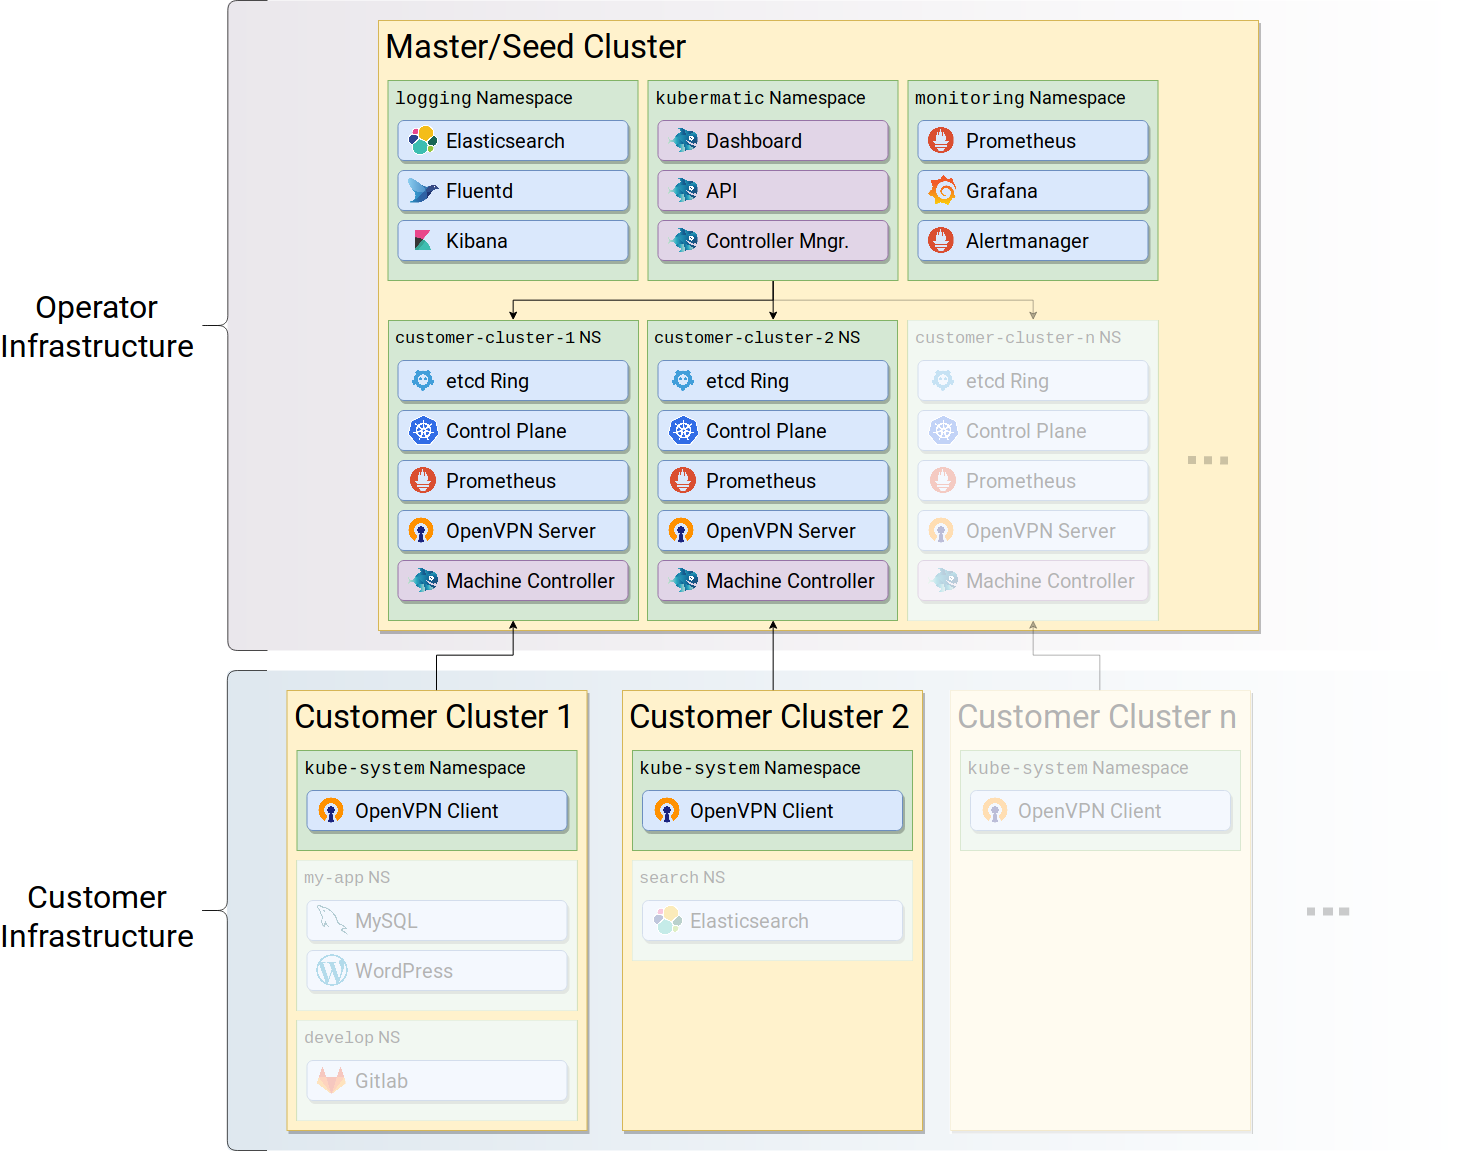
\includegraphics[width=1\textwidth, left]{media/05/kkp}
    \caption{"Kubermatic architecture, combined master seed" by Kubermatic GmbH CC BY 4.0}
    \label{fig:kubermatic}
\end{figure}

Another concept is the seed cluster, in which among other parts, the control-plane of a kubernetes cluster, that was created via KKP, lives.
As \autoref{fig:kubermatic} shows, the seed cluster can be the same as the master, but it is not mandatory.
Especially for large scale deployments it is recommended to run several independent seed clusters.
Thus, only worker nodes have to be created and connected.
Virtual machines are created via a supported provider, which are then provisioned by KKP and added as nodes.
\\
The master as well as the seed cluster should be operated in a High Available setup.
This offers the advantage that the Kubernetes control plane of the customer cluster is automatically a High Available setup.

\section{KubeLB}\label{sec:KubeLB}

The idea behind KubeLb is to adopt Concepts of KKP for LoadBalancing in multicloud, on-prem and edge Kubernetes environments.

As mentioned in \autoref{sec:ExternalLoadBalancer}, LoadBalancers needs to be integrated manually to every cluster.
This is especially needed for bare metal environments, where no cloud provider solution is available.
The already existing open source solutions for the implementation of the LoadBalancer, target single Kubernetes clusters, and are not designed for a highly dynamic multi cloud infrastructure.
\\
%Describe needed features
The key feature is to make LoadBalancing easily integrated and available in many, dynamically created and deleted, Kubernetes clusters.
%Compare features with open source stuff

%Describe possible features




%Customers?

